\documentclass{article}
\usepackage{graphicx} % Required for inserting images
\usepackage{caption} % Various image caption utilities
\usepackage{float}
\usepackage{lipsum}
\usepackage{nameref}
\usepackage{minted}
\usepackage{amsmath}
\usepackage[most]{tcolorbox}
\usepackage{geometry}
\usepackage{subcaption}
\usepackage{mdframed}
\usepackage{gensymb}

 \geometry{
 a4paper,
 total={6in,8in},
 left=1in,
 top=1in,
 bottom=1.5in
 }
\definecolor{LightGray}{gray}{0.9}


\title{Dynamic Optimization of Health Facility Accessibility: A Voronoi Diagram Approach}
\author{Alexander Xu}

\begin{document}

\maketitle

\begin{abstract}
This research explores the application of Voronoi diagrams in modeling and optimizing access to public health facilities. It begins with basic modeling of population distribution across an area using a set of points and cells. By overlaying population data onto these cells, the study provides insights into facility loading and imbalances among facilities. Recognizing the complexity of real-world scenarios, the research introduces an enhanced scoring system that incorporates population distribution, geographic characteristics, patient choice variability, and other risk factors such as health conditions and facility criticalness. These refinements enable a more accurate assessment of facility performance and accessibility.

The research further develops dynamic optimization algorithms, including weighted k-means clustering and iterative adjustments, to balance key physical properties, particularly population distribution across facilities. Using real-world data from Atlanta, Georgia, the study demonstrates the practical applicability of these approaches in identifying and potentially mitigating disparities in facility access. Throughout the research, we programmed the improved Voronoi diagram model using Matplotlib in Python and included raw code for reference and use by others. Finally, we explore basic ideas for alternative algorithms to improve population imbalance checks and create "forces" to move the facilities.
\end{abstract}


\section{Introduction}
\subsection{Health Facilities Today}
The demand for public health systems around the globe continues to rise. Indeed, population aging, the increased incidence of chronic disease, and a higher demand for mental health services are all expected to cause a rise in patient volumes \cite{aha-rise}. At the same time, public health systems face several issues today. One is wait times. A report by AANP finds that $26\%$ of patients wait two or more months for care in the United States, while $40\%$ of survey respondents experienced a "longer than reasonable" wait for health care \cite{aanp-wait}. Another study on Canada's public health system found that patients waited a median of 78 days to receive care \cite{canada-wait}.  Another is disparities in access, particularly in demographic determinants. There is growing recognition of implicit biases affecting social determinants of health and healthcare quality, particularly impacting minority and economically disadvantaged communities \cite{race-disparity}. Systems are also often not particularly optimized. For instance, during COVID, studies found that while some ICU units were overloaded, other nearby hospitals had excess capacity \cite{covid-imbalance}. Addressing these issues requires a combination of operational research and open dialogue to develop effective solutions.


\subsection{Understanding Voronoi Diagrams}
Voronoi diagrams, first formally introduced by Georgy Voronoi in 1908, are geometric structures that partition space based on proximity to a given set of \textit{source points} or \textit{seeds}. These diagrams consist of \textbf{cells} and \textbf{edges}. Each source point is associated with a cell, encompassing all the points in the space closer to that point than any other. The boundaries between these cells form the edges of the diagram. As a result, geometrically, the cells are polygons, and the edges are straight line segments.

A point $p$ belongs to the cell (or edge) of a source point $i$ from the set of source points $S$ if:
$$
\forall j \in S,  i \neq j, \mathrm{dist}(p, i) \leq \mathrm{dist}(p, j)
$$

In simpler terms, point $p$ belongs to the cell of source point $i$ if it is closer to $i$ than to any other source point $j$ in the set $S$. 

Checking what cell a point is in would run in $\mathrm{O}(n)$ time complexity, where the number of iterations is the size of $S$.

To further illustrate the idea of a Voronoi diagram, we can ask what the Voronoi diagram of just two source points would be. It is not hard to see that the defining boundary between the Voronoi cells is the perpendicular bisector between the two points \textbf{(Figure \ref{fig:voronoi-diagram-of-2})}:

\begin{figure}[h!]
\centering
\captionsetup{justification=centering,width=.9\linewidth}

\includegraphics[trim={0 10cm 0 6cm},clip,scale=0.30]{voronoi_bisector1.pdf}
\caption{Between two points, the edge defining the Voronoi diagram is the perpendicular bisector between the points.}
\label{fig:voronoi-diagram-of-2}
\end{figure}

As a result, more generally, the Voronoi diagram for any set of source points is just some combination of their $n \choose 2$  perpendicular bisectors \textbf{(Figure \ref{fig:voronoi-diagram-example})}.

\begin{figure}[H]
\centering
\captionsetup{justification=centering,width=0.8\linewidth}
\includegraphics[clip, scale=0.11]{voronoi_example2.png}
\caption{A Voronoi Diagram can look complex, but on closer inspection, all the edges are a section of some perpendicular bisector}
\label{fig:voronoi-diagram-example}
\end{figure}

So far, by the definition of a Voronoi cell, our idea of perpendicular bisectors works great. However, suppose we want to model systems with more conditions. In that case, we may want to use a \textbf{weighted Voronoi diagram} where we modify the dist function, which is currently Euclidean distance, to some other function. 
\vspace{15pt}



\section{Modelling Health Systems with Voronoi Diagrams}
\subsection{Basic Modelling with Population}

Imagine that source points represent the positions of some kind of facility. Then, by constructing a Voronoi diagram, we would know the region closest to every particular facility. In an idealistic, unconstrained, and efficient world, we can imagine that without fail, any person in the Voronoi cell of facility $i \in S$ would always access facility $i$, and any person outside of the cell would never access facility $i$.

Now let $P$ be the distribution of a population across an area, a set of points with populations. By overlaying a Voronoi diagram on $P$, we can define $P_i$ as the set of points in $P$ that are in the cell of facility $i$. Also, for convenience, we define a function $pop$ such that: 
\begin{itemize}
    \item if point $p \in P$ is inputted, $pop(p)$ returns the population at point $p$.
    \item if facility $i \in S$ is inputted, $pop(i)$ returns the population in the Voronoi cell of $i$. Using the previous definition:
    $$
    pop(i) = \sum_{p\in P_i} pop(p)
    $$
\end{itemize}
For $pop(i)$ people, facility $i$ is closer to them than any other facility, so the number of people that would go to facility $i$ or the \textbf{load} of facility $i$ would be $pop(i)$. 

To demonstrate, let's start with a system of three facilities and construct its Voronoi diagram. Then, let's create a sample $P$, which is a set of points and populations.

\begin{figure}[H]
\begin{subfigure}[t]{0.5\textwidth}
  \centering
  \captionsetup{justification=centering}
    \includegraphics[trim={0 10cm 0 6cm},clip,scale=0.25]{three_system_demonstration1.pdf}
  \caption{Voronoi diagram of 3 facility system}
  \label{fig:sub1}
\end{subfigure}%
\begin{subfigure}[t]{0.5\textwidth}
  \centering
  \captionsetup{justification=centering}
    \includegraphics[trim={0 5cm 0 5cm},clip,scale=0.19]{grid_points_for_3.pdf}
  \caption{Sample P, set of population points (can be grid or not depending on sample data)}
  \label{fig:sub2}
\end{subfigure}
\end{figure}

When we overlay P on the Voronoi diagram, we get a sense of points of population that will go to each facility, because they are contained in its cell:

\begin{figure}[H]
\centering
\captionsetup{justification=centering}
\includegraphics[trim={0 9cm 0 6cm},clip,scale=0.30]{three_system_demonstration_overlay.pdf}
\caption{Overlaying P on the Voronoi diagram}
\label{fig:demonstration-3-2}
\end{figure}

Each point in P is in one of the cells of the Voronoi diagram (with real data, positions are usually floating-point numbers, so a point being on an edge is exceedingly rare). We can add together the points in each cell to obtain an "expected" population going to each facility, $pop(i)$ (we improve on the expected population in \textbf{2.4}). 

Of course, with 3 facilities, we would have 3 Voronoi cells and $P_1, P_2, P_3$. From Figure 5, in the current system: 

\begin{itemize}

\item $pop(facility_1) = \sum\limits_{p \in P_1} pop(p) = 500 + 450 + 400 + 450 + 400 + 350 + 400 + 350 + 300 + 350 + 300 + 300 = \mathbf{4550} \implies $ \textbf{The load of facility 1 is 4550 people.}

\item $pop(facility_2) = \sum\limits_{p \in P_2} pop(p) = 350 + 300 + 250 + 300 + 250 + 200 + 250 + 200 + 150 + 100 = \mathbf{2350} \implies $ \textbf{The load of facility 2 is 2350 people.}

\item $pop(facility_3) = \sum\limits_{p \in P_3} pop(p) = 250 + 200 + 150 + 250 + 200 + 150 + 100 + 50 + 250 + 200 + 150 + 100 + 50 + 150 = \mathbf{2250} \implies $ \textbf{The load of facility 3 is 2250 people.}

\end{itemize}

This hints at an important idea:  \textbf{we can balance and improve "access" for all facilities by balancing the value of $P_i$ for all the facilities $i \in S$.}

It is not hard to see that the optimal solution is when $pop(facility_i) = \frac{\sum_{p\in P}{pop(p)}}{n}$, an even split of the population given $n$ is the number of facilities calculated by the average. In the system above, the average would be $\mathbf{3050}$. Evidently, facility 1 could be described as \textit{overloaded} while facilities 2 and 3 could be described as \textit{underloaded}.

\subsection{Programming a Voronoi Diagram Model}

\textbf{We aim to write an easily modifiable program that can draw Voronoi diagrams and calculate facility populations. This section will focus on the programming aspect of creating such a program, which may help to understand the visuals and process in the next sections but can be skipped.} 

We start with a program to display basic Voronoi diagrams. The program utilizes Matplotlib in Python to create visuals and graphs, and heavily uses SciPy's spatial library to do efficient Voronoi computations. The source points represent the positions of facilities (in the code, for convenience and visuals, it is useful to add four distant ghost points in the far corners).


\begin{minted}[frame=lines, framesep=2mm, bgcolor=LightGray,
mathescape, linenos, breaklines]{python} 
import numpy as np
import matplotlib.pyplot as plt 
from scipy.spatial import Voronoi, Delaunay, voronoi_plot_2d

def startVoronoi(source_points, bounding_box, refresh_time):
    #modify source points to include distant ghost points so the actual facilities' cells won't be "infinite" in size
    upd_source_points = np.append(source_points, [[999,999], [-999,999], [999,-999], [-999,-999]], axis = 0)
    plt.ion()
    
    while (True):
        vor = Voronoi(upd_source_points)
        voronoi_plot_2d(vor, ax=ax)
        
        ax.set_xlim(bounding_box[0],bounding_box[1]) 
        ax.set_ylim(bounding_box[2],bounding_box[3])
        
        regions = vor.regions
        for i in range(len(regions)):
            region = regions[i]
            polygon = [vor.vertices[i] for i in region]
            
            ax.fill(*zip(*polygon), alpha=0.4, data={"hello": 1}, facecolor="#d1ffbd")

            if (i < len(source_points)):
                ax.annotate("Index: " + str(i), (source_points[i, 0], source_points[i, 1]))
        
        plt.pause(refresh_time)
        ax.clear()
        
pop_points = np.array([])
bounding_box = np.array([0., 30.5, 0., 30.5]) #x_min, x_max, y_min, y_max
source_points = np.array([(1, 1), (6, 10), (25, 2), (15, 23), (6, 7)])
fig, ax = plt.subplots()
refresh_time = 5

startVoronoi(source_points, bounding_box, refresh_time)
\end{minted}

After implementing the Voronoi drawing and cell coloring, we obtain:

\begin{figure}[H]
    \centering
    \captionsetup{justification=centering}
    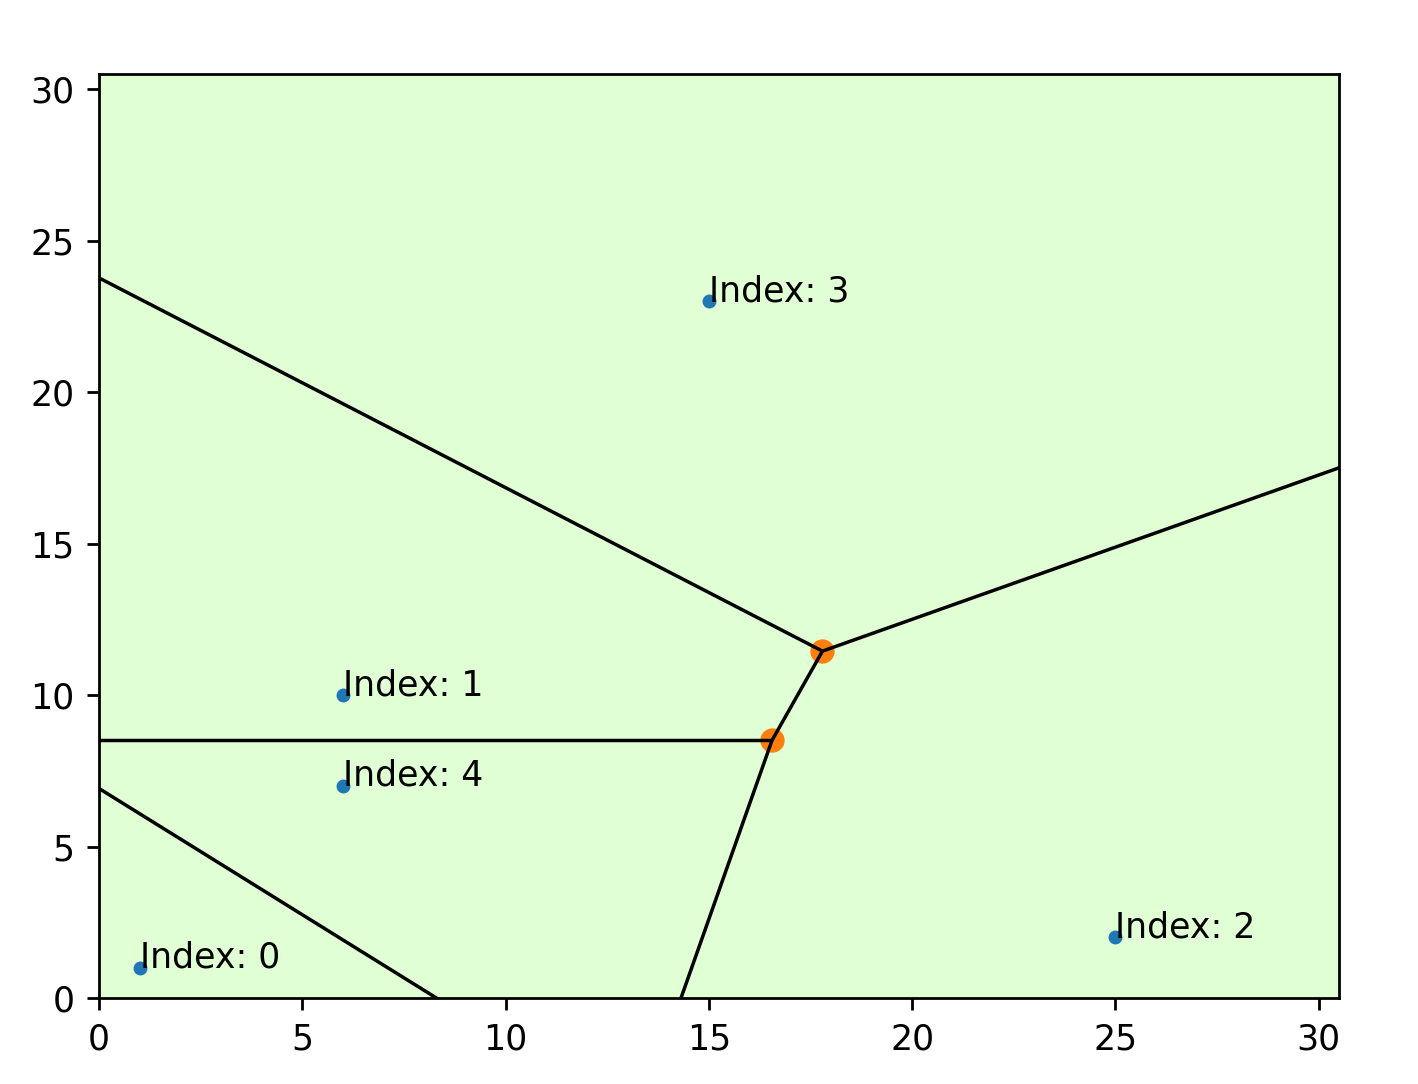
\includegraphics[clip,scale=0.20]{voronoi_draw_demo.png}
    \caption{Result generated from program}
    \label{fig:mid-interface}
\end{figure}

We create the population distribution $P$, and calculate the average of all populations, which we described as the most "optimal" solution.

\begin{minted}[frame=lines, framesep=2mm, bgcolor=LightGray,
mathescape, linenos, breaklines]{python} 
pop_list = []
pop_avg = 0

for i in range(0, 5):
    for j in range(0, 5):
        pop_val = 45 - 5 * (i + j)
        pop_list.append([7 * i, 7 * j, pop_val])
        
        pop_avg += pop_val

pop_avg /= len(source_points)

pop_points = np.array(pop_list)
\end{minted}

We can plot this $P$ in a scatterplot on Matplotlib:

\begin{figure}[H]
    \centering
    \captionsetup{justification=centering}
    \includegraphics[clip,scale=0.20]{plot_P_1.png}
    \caption{Plotting P in Matplotlib}
    \label{fig:mid-interface}
\end{figure}

We write a function to calculate the population/load for each facility (when we get to algorithms this will be recalculated for each iteration):

\begin{minted}[frame=lines, framesep=2mm, bgcolor=LightGray,
mathescape, linenos, breaklines]{python} 
def recomputePopulations(pop_points, upd_source_points):
    #remove ghost points from calculation
    upd_source_points = upd_source_points[0:-4]
    
    source_point_pops = np.zeros(len(source_points))
    
    for point in pop_points:
        p_x = point[0]
        p_y = point[1]
        
        min_dist = 1e12
        min_index = -1
        for i in range(0, len(source_points)):
            source_x = upd_source_points[i, 0]
            source_y = upd_source_points[i, 1]
        
            dist = (source_x - p_x)**2 + (source_y - p_y)**2
            if (dist < min_dist):
                min_dist = dist
                min_index = i

        source_point_pops[min_index] += point[2]
    
    return source_point_pops
\end{minted}

At this step, we updated the visual diagram to label each facility based on its population and color each cell based on the ratio of population and $avg$ so that the current state of the system is clear. After all is said and done, we have a view like: 

\vspace{10pt}
\begin{figure}[h!]
    \centering
    \captionsetup{justification=centering}
    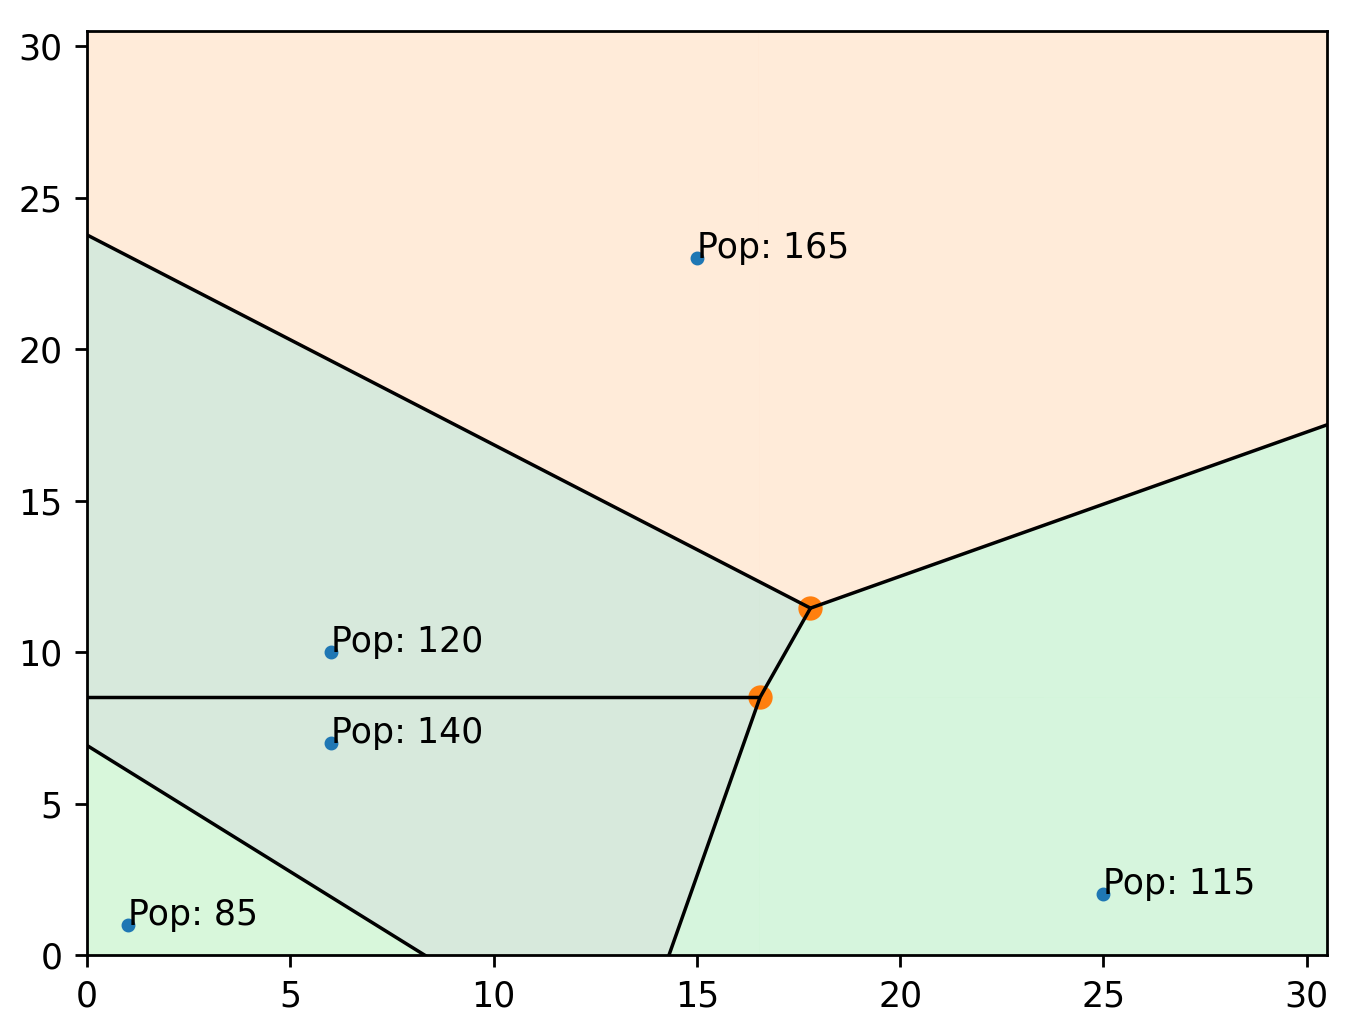
\includegraphics[clip,scale=0.24]{voronoi_draw_final.png}
    \caption{Interface with labeled facilities and colored cells for modelling a system.}
    \label{fig:final-interface}
\end{figure}
\vspace{10pt}

Now, given a system of facilities and a population distribution, we are able to run this program to make a general visual model of underloaded and overloaded facilities. Cells are colored based on the ratio of the population in the cell to the average. Overloaded facilities are marked by orange/red cells, while good or underloaded facilities are marked by white/green cells. 

\subsection{Adding Factors in the Model}
Simply considering population ignores a lot of factors that should be considered. Instead of basing our model off of $pop(i)$, simply the population in each Voronoi cell, let's create a new score metric. Specifically, we create an $S_i$ that will define a \textit{score} for each facility based on a combination of factors. In the code, we would modify the \textit{recomputePopulations} functions to be a \textit{recomputeScores} function. We will define a higher $S_i$ to mean a worse loaded facility based on a variety of factors, 


To start, we'll include the $pop(i)$ in the calculation of $S_i$ so $S_i = pop(i) + factors$. We proceed to identify some of those factors.

\subsubsection*{1. Distance from Facility}
A major flaw with only considering the population in a Voronoi cell is that the distance from the facility is not considered. While two Voronoi cells can have the same population, if one is significantly larger than the other and the actual facility is far away from the population in the cell, the facility is not optimized. 
Let $r$ be the maximum \textit{acceptable} distance. $r$ may be the same across all facilities, or we may define a unique $r$ for a specific facility if, for instance, a facility saw more elderly people who couldn't travel as far. 

\begin{figure}[h!]
    \centering
    \captionsetup{justification=centering,width=.9\linewidth}
    \captionsetup{justification=centering}
    \includegraphics[trim={0 4cm 0 4cm},clip,scale=0.26]{three_system_circles.pdf}
    \caption{The circles show the area a distance of at most $r$ around each facility. Each facility should ideally be at most $r$ distance away from the population in its Voronoi diagram, which drawing the circles shows.}
    \label{fig:final-interface}
\end{figure}

From the set $P_i$, we obtain the subset of points that would be outside of this radius $r$:

$$
P_{i,r} = \{p \in P_i \mid \mathrm{dist}(p,i) >r\}
$$

The population outside of the circle of acceptable distance $r$ would then be:

$$
outPop_r(i) = \sum_{p \in P_{i, r}} pop(p)
$$

In our score $S_i$, we can now include $outPop_r(i)$ in the model, giving $S_i = pop(i) + outPop_r(i)$. This is equivalent to counting each person outside of the distance $r$ twice, penalizing a facility for having more population outside of the $acceptable$ area.

\subsubsection*{2. Fuzziness in Patient Choices}
We note that if a patient is sufficiently close to two or more facilities, they may have a "choice" on which facility to choose. Let's say that if a person is at most a distance $c$ away from facility $i$, there is a probability $\omega$ they will come to $i$. Equivalently, we can create a set $P_{i, c}$ which defines all points in $P$ but not in $P_i$ with a distance of at most $c$ to $i$: 

$$
P_{i, c} = \{p \in P \setminus P_i \mid \mathrm{dist}(p, i) \leq c\}
$$

Then, we calculate the population coming from other Voronoi cells to facility $i$ to be:

$$
extPop_c(i) = \omega\left(\sum_{p \in P_{i, c}} pop(p)\right)
$$

We add this new external population, $extPop_c (i)$, to the score $S_i$, so we have:

\begin{gather*}
    S_i = pop(i) + outPop_r(i) + extPop_c(i)\\
\end{gather*}

\subsubsection*{3. Possible Multiplicative Properties: Risk and Service}

Another factor we have not yet considered is the criticalness of the facility and the conditions of its patients. For instance, a facility in an area with more elderly people, or an area with a statistically significant number of people with a condition, would likely see more patients who need care. We can define an $r_i$ as the \textit{risk} of facility $i$, a blanket term for a scale based on the conditions and demographics of people in the area, similar to 
health risk models used in health insurance but applied to a collective ($https://pmc.ncbi.nlm.nih.gov/articles/PMC2990501/$). There are a few ways of determining a "risk" for facility $i$:

\begin{itemize}
    \item We create a model for risk combining factors like age,  rates for health conditions like diabetes, or income. Using other demographic factors like race in the model is more questionable, as trends between health and race are often correlation instead of causation. 
    \item If we already have historical data on the actual number of people using the facility or in the backlog, say that's $N$, then $N$ will be a percentage of $pop(i)$. Comparing the ratios $\frac{N}{pop(i)}$ for $i$ across the facilities, we can say that a facility with a significantly higher ratio has higher "risk", as a higher percentage of the population using a facility signifies higher demand and "risk".
    \item Similar to the last one, if we have historical data instead on the wait times of the facility, then we could compare the wait time $w$ to $pop(i)$. A facility with a significantly higher ratio has higher "risk", as wait times are also indicative of demand.
\end{itemize}

(https://pmc.ncbi.nlm.nih.gov/articles/PMC10527840/)

In theory, given a risk $r_i$, we conclude with our model for $S_i$: 

\begin{tcolorbox}[colback=white]
\begin{equation*}
    \begin{split}
        S_i &= r_i \left( pop(i) + outPop_r(i) - extPop_c(i)\right) \\
            &= r_i \left( pop(i) + \sum_{p \in P_{i, r}} pop(p) - \omega\left[\sum_{p \in P_{i, c}} pop(p)\right] \right) \\
    \end{split}
\end{equation*}
\vspace{1.5pt}
\end{tcolorbox}


\subsection{Conclusions on Modelling}
In this project, we developed a comprehensive model to evaluate and optimize access to facilities based on population distribution and other critical factors. Initially, we visualized the system by leveraging Voronoi diagrams to partition the population among facilities and color-coded cells based on the ratio of the population to an average threshold. This provided an intuitive and effective way to identify overloaded and underloaded facilities.

Building on this foundation, we introduced $S_i$ to quantify facility performance and expectations. These metrics incorporated population data and additional factors, refining the model to reflect real-world complexities better. By considering distance, external population contributions, and multiplicative risk properties, we accounted for a facility's geographical and demographic challenges and its capacity to support surrounding areas.

Through iterative enhancements, including penalizing facilities with populations beyond acceptable distances and rewarding those that support others, the model captured nuanced interactions between facilities and the populations they serve. Furthermore, integrating risk factors like demographics, health conditions, and historical usage data allowed for more precise assessments and informed decision-making.

The result is a robust system that not only highlights disparities in facility access but also suggests actionable improvements. These insights can drive strategic planning, optimize resource allocation, and promote equity in facility accessibility, addressing critical challenges in public health, urban planning, and resource distribution.

\vspace{15pt}
\section{Voronoi Diagram Optimization Algorithms}

Building on our framework for modeling facility accessibility using Voronoi diagrams, we now turn our attention to dynamic optimization algorithms aimed at balancing key physical properties, particularly population, within Voronoi cells. Given an initial system comprising population points and facility positions, the objective is to iteratively adjust facility locations such that the population distribution across the Voronoi cells becomes more equitable. This involves developing algorithms that evaluate the imbalance in population densities and reposition facilities over successive iterations to reduce discrepancies. We seek to derive a systematic process that converges toward an optimized configuration where no facility is overloaded relative to its neighbors, ensuring a fair and efficient system.

\subsection{K-Means Clustering and Lloyd's Algorithm}

\textit{\textbf{K-means}} is an unsupervised machine-learning algorithm for clustering data closely linked to Voronoi diagrams, as each cluster is defined as a Voronoi cell. Much like what we're trying to achieve, the k-means algorithm tries to partition $n$ points in $k$ cells iteratively equally.

The key idea is that at every iteration, given the population points contained in the cell of facility $i$ ($P_i$), we continually move the facility to the \textbf{centroid} of the population. 

We start by showing generic K-means clustering, which works in a system of points of equal weight.

\subsubsection*{Generic K-means Clustering}
Like the way we created $P$ and $P_i$, let $G$ be a set of points with only location, and without another property like population because all points are equally weighted. Keeping with the terminology of "facility", let $F$ be the set of facility positions. $G_i$ represents the set of points in G contained in the cell of facility $i$ at $F_i$. 

At each iteration, for each facility $i$ in $F$, we need to calculate its new position, which, by K-means, is the centroid of all the points in $G_i$. This means taking the average of the values $x$ of $G_i$, which is $centroid_x$, and taking the average of the values $y$ of $G_i$, which is $centroid_y$. Thus, the new position of the facility $i$, which is equal to the centroid of the points in $G_i$, can be expressed as:

\begin{gather}
    F_{i, x} = centroid_x = \frac{1}{|G_i|} \sum_{g \in G_i}{g_x}\\
    F_{i, y} = centroid_y = \frac{1}{|G_i|} \sum_{g \in G_i}{g_y}
\end{gather}

Note that after each iteration, the points have shifted, and so have the Voronoi diagrams. As a result, after each iteration, it is possible that $G_i$ has changed, so we need to recalculate $G_i$ during each iteration.

\subsubsection*{Weighted K-means With Population}

Returning to our system with facilities and population points, the points are \textit{not} equally weighted. Instead of computing the centroid of a group of equal points, we now compute their \textbf{weighted} centroid, which accounts for the population associated at each point. In this method, the position of a point contributes to the centroid proportionally to its population. As a result, facilities are "pulled" closer to areas with a higher population. Recall generally that the weighted average of $n$ terms with weight $w_i$ is:

$$
W = \frac{\sum_{i=1}^{n}{w_iX_i}}{\sum_{i=1}^{n}w_i}
$$

We know that the weights are the populations of the points in $P_i$, the weighted average of the points in $P_i$, and we defined the population of all the points in the cell of facility $i$, $P_i$, as  $\sum_{p \in P_i} pop(p) = pop(i)$. Thus, the new centroid of facility $i \in F$ at each iteration is:

\begin{gather}
    F_{i, x} = centroid_x = \frac{1}{pop(i)} \sum_{p\in P_i} \left( p_x \cdot pop(p) \right) \\
    F_{i,y} = centroid_y = \frac{1}{pop(i)} \sum_{p \in P_i} \left( p_y \cdot pop(p) \right)
\end{gather}

This gives us the weighted centroid of the points in $P_i$. At this point, we have a pretty good algorithm for balancing pure population in each facility/cell. Now, we now add on new constraints that we discussed in our model. For one, how do we now incorporate the maximum distance from the facility into a further modified k-means algorithm? Another is, how do we handle fuzzier choices where a person sufficiently close to multiple facilities and can choose one?

\subsubsection*{K-means With Constrained Distance from Facility}

Recall that in the model we created in \textbf{Section 2}, we noted that while the population in the cell of a facility might be balanced, the facility may be very far away from the actual population. We suggested that we define a function $outPop_r(i)$ that gives the population $pop(i)$ outside of the acceptable $r$ range around the facility $i$ (effectively in the circle $(x-F_{i, x})^2 + (y-F_{i, y})^2 = r^2$). As a baseline, we said that these people would be weighted $k = 2$ times as much as people within the range. Thus, we could employ a modified version of our weighted centroid function. The sum of the total weights, $w_{tot}$, which was previously just the sum of all the populations in the cell, $pop(i)$, is now:

\begin{align*}
    w_{tot} &= pop(i) + outPop_r(i) \\
            &= \sum_{p \in P_i} \left( pop(p) \cdot \begin{cases}
                 1 & p \notin P_{i, r} \\
                 2 & p \in P_{i, r} 
                \end{cases}
            \right)
\end{align*}

Note that the equation for $w_{tot}$, is just the score $S_i$ without the external population $extPop_c(i)$, which we'll include later. Now, the new centroid of facility $i \in F$ after each iteration is:

\begin{gather}
F_{i, x} = centroid_x = \frac{1}{w_{tot}} \sum_{p \in P_i} \left( p_x \cdot pop(p) \cdot \begin{cases}
                 1 & p \notin P_{i, r} \\
                 2 & p \in P_{i, r}
                \end{cases} \right) \\
F_{i, y} = centroid_y = \frac{1}{w_{tot}} \sum_{p \in P_i} \left( p_y \cdot pop(p) \cdot \begin{cases}
                 1 & p \notin P_{i, r} \\
                 2 & p \in P_{i, r}
                \end{cases} \right)
\end{gather}



\subsubsection*{External Populations and Fuzziness}

In the model we created in \textbf{Section 2}, we saw that if a person was close enough to a facility, $i$, even though they may be closer to another facility (in a different cell), $j$, they still had a chance of visiting facility $i$ over $j$. We defined the probability of a person "breaking" the norm and going to a different facility as $\omega$, and we said that a person has a chance of going to a different facility if a person is within a distance of $c$ away from the facility while being in a different facility. We say that the population inside $P_{i, c}$ (people outside of cell $i$ but within the range $c$), is weighted $\omega$ times as much as people inside the cell $i$ and the acceptable $r$ range we discussed in the previous subsection. The sum of the total weights, $w_{tot}$, is then:

\begin{align*}
    w_{tot} &= pop(i) + outPop_r (i) + extPop_c(i) \\
            &= \sum_{p \in P_i} \left( pop(i) \cdot \begin{cases}
                 1 & p \notin P_{i, r} \\
                 2 & p \in P_{i, r} 
                \end{cases}
            \right) + w\sum_{p \in P_{i, r}} pop(p)
\end{align*}

Thus, the new equation for the centroid of facility $i \in F$ after each iteration is:

\begin{gather}
F_{i, x} = centroid_x = \frac{1}{w_{tot}} \left( \sum_{p \in P_i} p_x \cdot pop(p) + \sum_{p \in P_{i, r}} p_x \cdot pop(p) + w\sum_{p \in P_{i, c}} p_x \cdot pop (p) \right)\\
F_{i, y} = centroid_y = \frac{1}{w_{tot}} \left( \sum_{p \in P_i} p_y \cdot pop(p) + \sum_{p \in P_{i, r}} p_y \cdot pop(p) + w\sum_{p \in P_{i, c}} p_y \cdot pop (p) \right)
\end{gather}

In this way, we consider more of the fuzziness in the system and the choices that people make. Later on, we also make the system fuzzier by breaking up a single population point into many to more accurately depict density.


\pagebreak

\section{Applications to Cities}
We now seek to see how our model and specialized balancing algorithm work on real data. Looking at the Atlanta area, we extracted population data in 37 zips. Each row of data has the ZIP code, the population, the latitude, and the longitude. We also noted 10 public health facilities. The ZIP data are population points that are distributed across the area, and the facilities are marked by the red points in \textbf{Figure 9}.

\begin{figure}[H]
    \centering
    \captionsetup{justification=centering,width=.9\linewidth}
    \captionsetup{justification=centering}
    \includegraphics[trim={0 0cm 0 0cm},clip,scale=0.12]{pop_graph_with_fac.png}
    \caption{Facility locations are marked at the red points.}
    \label{fig:pop_points with facilities}
\end{figure}

The scoring model is visualized by the Voronoi diagram and two circles of radius $r$ and $c$ around each facility. For this system, we let $r = 0.1 \degree \ \textrm{lat/lon} \approx 7 \ \textrm{miles}$ and $c = 0.05 \degree \ \textrm{lat/lon} \approx 4 \ \textrm{miles}$. Then, our system can be represented chaotically as: 

\begin{figure}[H]
    \centering
    \captionsetup{justification=centering,width=.9\linewidth}
    \captionsetup{justification=centering}
    \includegraphics[trim={0 0cm 0 0cm},clip,scale=0.12]{chaotic-elements.png}
    \caption{Elements including the Voronoi diagram and $r$ and $c$ range circles all added.}
    \label{fig:final-interface}
\end{figure}

In \textbf{Figure 10}, the Voronoi diagram is drawn. Also, green circles of radius $r$ and blue circles of radius $c$ are constructed around each population point. Only computing the populations in the cell of each facility, we get the following results:

\begin{figure}[H]
    \centering
    \captionsetup{justification=centering,width=.9\linewidth}
    \captionsetup{justification=centering}
    \includegraphics[trim={0 0cm 0 0cm},clip,scale=0.12]{atlanta_pop_voronoi.png}
    \caption{Facility locations are marked at the red points.}
    \label{fig:final-interface}
\end{figure}
\begin{center}
\begin{tabular}{ | c | c | c | }
 \hline
 Id & Facility Name & Population \\
 \hline
 1 & Grady Memorial Hospital & 12083 \\ 
 2 & Asa G. Yancey Health Center & 96560 \\  
 3 & Brookhaven Health Center & 273315 \\
 4 & Camp Creek Comprehensive Care Center & 75615 \\
 5 & Cascade Outpatient Center & 94221 \\
 6 & East Point Health Center & 49444 \\
 7 & Kirkwood Health Center & 60502 \\
 8 & Kee + White Outpatient Center & 86215 \\
 9 & North Fulton Health Center & 125004 \\
 10 & Emory Executive Health Center & 65685 \\
 \hline
\end{tabular}
\end{center}

\vspace{12}
Some data, particularly near the edges, may be incomplete due to populations and facilities located outside the analyzed area. However, the methodology remains valid for demonstrating the algorithm. To observe the level of \textit{disparity} or \textit{unbalancedness} in the current system, we can take the standard deviation, which is $\sigma = \sqrt{\frac{\sum(x_i - \mu)^2}{N}} = \mathbf{66437.668}$.

Instead of population, we can now calculate the scores, $S_i$, for each facility. The following program gives an example of how the score could be calculated, incorporating the original population, adding weight to the population outside of the cell, and external population outside of the cell.

\vspace{12}

\begin{minted}[frame=lines, framesep=2mm, bgcolor=LightGray,
mathescape, linenos, breaklines]{python} 
def recomputeScores(pop_points, upd_source_points):
    #remove ghost points from calculation
    upd_source_points = upd_source_points[0:-4]
    
    #stores the scores of each source point
    source_point_scores = np.array(np.zeros(len(upd_source_points))) 
    #stores the nearest source point (cell id) for each population point
    pop_sources = np.array(np.zeros(len(pop_points)), dtype=np.int16)
    
    #code to count normal population
    for i in range(0, len(pop_points)):
        p_x = pop_points[i, 2]
        p_y = pop_points[i, 3]
        
        min_dist = 1e12
        min_index = -1
        for j in range(0, len(upd_source_points)):
            source_x = upd_source_points[j, 0]
            source_y = upd_source_points[j, 1]
        
            #keep square for efficiency
            dist = (source_x - p_x)**2 + (source_y - p_y)**2
            if (dist < min_dist):
                min_dist = dist
                min_index = j

        source_point_scores[min_index] += pop_points[i, 1]
        pop_sources[i] = min_index
        
        #if out of range, the population holds double the weight 
        if (min_dist > r*r):
            source_point_scores[min_index] += pop_points[i, 1]
    
    
    #code to handle fuzziness, weighted omega
    for i in range(0, len(pop_points)):
        p_x = pop_points[i, 2]
        p_y = pop_points[i, 3]
        
        for j in range(0, len(upd_source_points)):
            source_x = upd_source_points[j, 0]
            source_y = upd_source_points[j, 1]
            
            dist = (source_x - p_x)**2 + (source_y - p_y)**2
            if (dist <= c*c and pop_sources[i] != j):
                source_point_scores[j] += omega * pop_points[i, 1]
        
    return [source_point_scores, pop_sources]
\end{minted}

On using the scores, we get updated results: 


\begin{figure}[H]
    \centering
    \captionsetup{justification=centering,width=.9\linewidth}
    \captionsetup{justification=centering}
    \includegraphics[trim={0 0cm 0 0cm},clip,scale=0.12]{atlanta_score_voronoi.png}
    \caption{Facility locations are marked at the red points.}
    \label{fig:final-interface}
\end{figure}
\begin{center}

\begin{tabular}{ | c | c | c | c | c | }
 \hline
 Id & Score & Population & Pop Outside Range $r$ & External Pop in $c$ (times $\omega=0.2$)\\
 \hline
 1 & 18779.4 & 12082 & 0 & 33482 \\ 
 2 & 127595.8 & 96560 & 20203 & 54164 \\  
 3 & 310310.4 & 273315 & 32560 & 22177 \\
 4 & 75615 & 75615 & 0 & 0 \\
 5 & 94221 & 94221 & 0 & 0 \\
 6 & 57651.6 & 49444 & 0 & 41038 \\
 7 & 68600.4 & 60502 & 0 & 40492 \\
 8 & 97801.6 & 86215 & 0 & 57933 \\
 9 & 142603 & 125004 & 17599 & 0 \\
 10 & 80027.2 & 65685 & 0 & 71711 \\
 \hline
\end{tabular}
\end{center}

From this data, we have that the standard deviation of facility scores was $\sigma = \mathbf{75285.446}$. Now, let us run the weighted k-means only considering population on this dataset and observe the population and population outside range $r$:

\begin{figure}[H]
    \centering
    \captionsetup{justification=centering,width=.9\linewidth}
    \captionsetup{justification=centering}
    \includegraphics[trim={0 0cm 0 0cm},clip,scale=0.12]{k-means-pop.png}
    \caption{Result after k-means with population reaches steady state ($\approx$ 8 iterations).}
    \label{fig:final-interface}
\end{figure}

\begin{center}
\begin{tabular}{ | c | c | c | c | }
 \hline
 Id & Facility Name & Population & Pop Outside Range $r$\\
 \hline
 1 & Grady Memorial Hospital & 28045 & 0 \\ 
 2 & Asa G. Yancey Health Center & 146268 & 0 \\  
 3 & Brookhaven Health Center & 108070 & 0 \\
 4 & Camp Creek Comprehensive Care Center & 75615 & 0 \\
 5 & Cascade Outpatient Center & 58302 & 0 \\
 6 & East Point Health Center & 69401 & 0 \\
 7 & Kirkwood Health Center & 78817 & 0 \\
 8 & Kee + White Outpatient Center & 108229 & 0 \\
 9 & North Fulton Health Center & 154293 & 0 \\
 10 & Emory Executive Health Center & 111604 & 0 \\
 \hline
\end{tabular}
\end{center}

From this data, we note two things. Firstly, the k-means algorithm has moved the facilities such that there is no population within each cell outside of a range $r$. This makes sense because k-means optimizes variance within a cell, though it shows that k-means is a viable solution for optimizing distance travel time for populations. Calculating the new standard deviation, we obtain $\sigma_{new} = \mathbf{37249.681}$. This marks a $\mathbf{44\%}$ reduction in standard deviation from $\mathbf{66437.668}$. 

Meanwhile, applying the score-based algorithm, we get the following results:

\begin{figure}[H]
    \centering
    \captionsetup{justification=centering,width=.9\linewidth}
    \captionsetup{justification=centering}
    \includegraphics[trim={0 0cm 0 0cm},clip,scale=0.12]{k-means-score.png}
    \caption{Result after k-means with score reaches steady state ($\approx$ 20 iterations).}
    \label{fig:final-interface}
\end{figure}

\begin{center}
\begin{tabular}{ | c | c | c | c | c | }
 \hline
 Id & Score & Population & Pop Outside Range $r$ & External Pop in $c$ (times $\omega=0.2$)\\
 \hline
 1 & 61527 & 61527 & 0 & 0 \\ 
 2 & 94687 & 94687 & 0 & 0 \\  
 3 & 148701 & 148701 & 0 & 0 \\
 4 & 75615 & 75615 & 0 & 0 \\
 5 & 58302 & 58302 & 0 & 0 \\
 6 & 82415 & 82415 & 0 & 0 \\
 7 & 87858 & 78817 & 0 & 45205 \\
 8 & 97801.6 & 86215 & 0 & 57933 \\
 9 & 107405 & 17405 & 0 & 0 \\
 10 & 169442 & 169442 & 0 & 0 \\
 \hline
\end{tabular}
\end{center}

The standard deviation of the score is $\sigma = \mathbf{33949.466}$, which marks a $\mathbf{54.9\%}$ reduction in deviation from $\mathbf{75285.446}$.

\section{Additional Thoughts}

This section includes alternative algorithms and ideas that might provide alternative solutions. Particularly, k-means rapidly approaches a local optimum, but how do we modify the algorithm to approach a global optimum? Along with k-means, I was looking at another algorithm using virtual forces to balance populations. A possible solution to k-means finding a global optimum is to combine the k-means algorithm with a virtual force algorithm, which I now show.

\subsection{Shifting Facilities}

Turning back to the system we introduced in \textbf{2.1}, we found that the population of facility 1 was 4550, facility 2 was 2350, and facility 3 was 2250. One way we could have "balanced" the system was to move facilities 2 and 3 closer to 1, effectively taking away some population from the Voronoi cell of cell 1.

In general, the load across facilities can be improved by moving facilities with less load toward facilities with more load. In a Voronoi diagram, this has the effect of \textit{squeezing} Voronoi cells, which in practice allows one facility to \textit{acquire} some of the population of another. Some questions arise from doing this too generally, which we'll discuss in $\mathbf{2.4}$. We make use of two main "properties" of shifting facility positions and Voronoi diagrams:
\vspace{6pt}
\begin{tcolorbox}
\centering
\textit{Squeezing}: Moving the points that are directly around $i$ (a.k.a Voronoi cells are adjacent) closer to $i$ decreases the size of the Voronoi cell of $i$ and the load on $i$.

\includegraphics[width=5cm,trim={0 12cm 0 8cm},clip]{voronoi_squeeze_1.pdf}
\includegraphics[width=5cm,trim={0 12cm 0 8cm},clip]{voronoi_squeeze_2.pdf}
\end{tcolorbox}
\vspace{4pt}
\begin{tcolorbox}
\centering
\textit{Insulation}: Moving a point $q$, that is not directly around $i$, towards a point $p$, that is directly around $i$ (a.k.a Voronoi cells are adjacent), along the vector $v_{pq}$, has no impact on the Voronoi cell of $i$ and the load on $i$.

\includegraphics[width=5cm,trim={0 10cm 0 9cm},clip]{voronoi_insulation_1.pdf}
\includegraphics[width=5cm,trim={0 10cm 0 9cm},clip]{voronoi_insulation_2.pdf}
\end{tcolorbox}
\vspace{6pt}


We aim to develop algorithms that optimize facility placement to achieve more balanced states. To formalize this, let \textit{\textbf{it}} represent the number of iterations of each algorithm needed to see results, and let \textit{\textbf{avg}} represent the average population of a facility, which we state is the "optimal" population for each facility.

\subsection{Extending Program to Handle Algorithmic Iteration}

\textbf{We aim to modify the program introduced in 2.2 to be able to test algorithms and iteratively shift the Voronoi diagram. This section will focus on the programming aspect of creating such a program, which may help to understand the visuals and process in the next sections but can be skipped.} 

In 2.2, we already wrote all the code to create the Voronoi diagram and redraw it, with the continuously repeating while loop and the \textbf{recomputePopulation} function. 

Now, We add a necessary helper function that will hold the algorithms we test. In general, our algorithms will generate a set of vectors that will be applied to shift the original positions of the vectors. 

\begin{minted}[frame=lines, framesep=2mm, bgcolor=LightGray,
mathescape, linenos, breaklines]{python} 
def algorithmGenerateVectors(upd_source_points, source_point_pops):
    #remove ghost points from calculation
    upd_source_points = upd_source_points[0:-4]
    
    apply_vectors = np.array(np.zeros((len(upd_source_points), 2)))
    
    #some modifications based on algorithm
    
    return apply_vectors
\end{minted}

We simply apply the vectors by adding them to the previous position of the facilities. This part is recomputed with each iteration.  


\begin{minted}[frame=lines, framesep=2mm, bgcolor=LightGray,
mathescape, linenos, breaklines]{python} 
calculated_vectors = algorithmGenerateVectors(upd_source_points, source_point_pops)
    
for i in range(len(calculated_vectors)):
    upd_source_points[i, 0] += calculated_vectors[i, 0]
    upd_source_points[i, 1] += calculated_vectors[i, 1]

    upd_source_points[i, 0] = bound(upd_source_points[i, 0], bounding_box[0], bounding_box[1])        
    upd_source_points[i, 1] = bound(upd_source_points[i, 1], bounding_box[2], bounding_box[3])
\end{minted}

Now, we essentially have all the pieces to test algorithms. 



\textbf{In testing algorithms}, we start with algorithms that are easier to implement and likely the first that come to mind. Some of these don't work very well at all, while others have very high \textit{\textbf{it}} values.

\vspace{12pt}
\subsection{Attractive Forces}

At every iteration, we find the facility with the highest population, call it $p$. Then, we find the facility with the smallest population that is directly next to $p$, call it $q$.

Our strategy is to move $q$ closer to $p$, so that the cell of $p$ will shrink and $q$ can \textit{acquire} some of the population from $p$. It makes sense for $q$ to move closer to $p$ along the vector $v_{qp}$. Using the unit vector, $\hat{v}_{qp} = \frac{v_{qp}}{|v_{qp}|}$, we could move $q$ a percentage, $per$, of $v_{qp}$, and limit the movement to at most $k_{max}$ towards $p$ (min is the shorter vector): 

$$q_{new} = q + \mathrm{min} (per\cdot v_{qp},\ k_{max} \cdot \hat{v}_{pq}) $$.

However, if the system is already balanced, we aim to ensure it remains stable. Indeed, if the populations of two cells are already well-balanced, shifting one facility toward the other might make it more imbalanced. As a result, it would probably help to limit movement according to $pop(p)$ and $pop(q)$ by some limiting function $L(p, q) \in [0, 1]$:

$$
q_{new} = q + L(p, q) \cdot \mathrm{min} (per\cdot v_{qp},\ k_{max} \cdot \hat{v}_{pq})
$$

A simple limiting function could be the complement of the ratio of $pop(q)$ and $pop(p)$. To limit movement further and prevent cases like "ping-ponging" where one facility bounces between two states, and balanced states devolve over time, we can take the function to a power $n$. Since L is bounded by $[0, 1]$, the result is that the movement at each iteration will always be less: 

\begin{equation}
L(p, q) = 1 - \frac{pop(q)}{pop(p)}
\end{equation}

\begin{equation}
L_n(p, q) = \left( 1 - \frac{pop(q)}{pop(p)} \right)^n
\end{equation}

Another idea for a limiting function is to replace $pop(q)$ with $avg$, which makes sense because $pop(p)$ needs to approach $avg$ anyway. We stop once the cell is "good enough", such as when the ratio of $avg$ and $pop(p)$ is greater than $0.9$ (or $pop(p)$ is less than $\frac{10}{9} \times avg$).


\begin{equation}
L(p, q) = \begin{cases} 
      0 & \frac{avg}{pop(p)} \geq 0.9 \\
      1 - \frac{avg}{pop(p)} & \frac{avg}{pop(p)} < 0.9 \\
   \end{cases}
\end{equation}

\subsubsection{Testing}

Starting from this example again:

\begin{figure}[H]
    \centering 
    \hfill 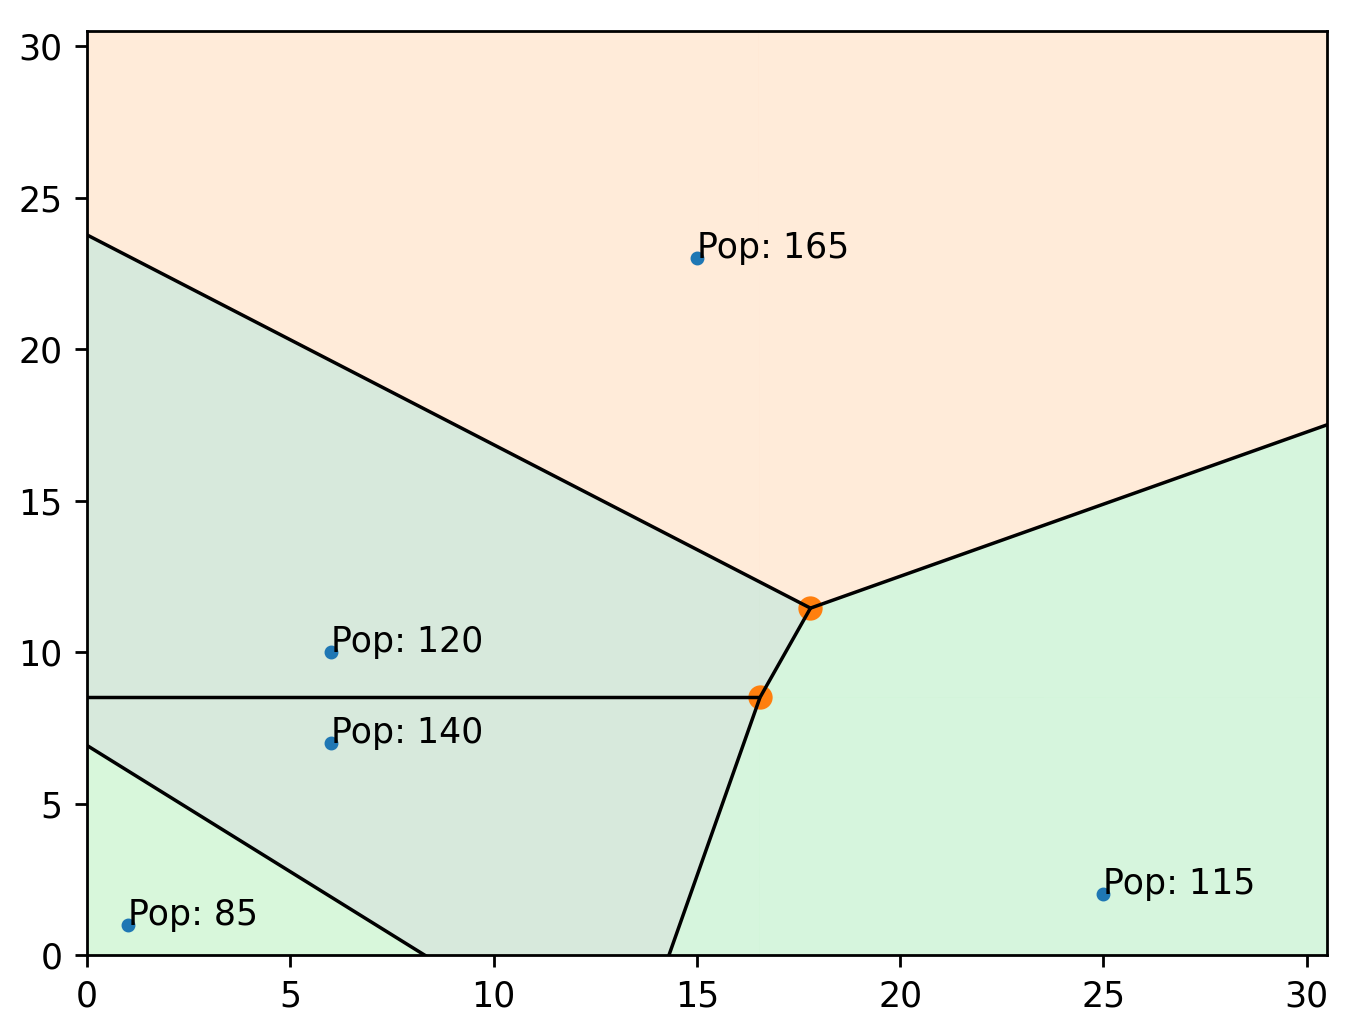
\includegraphics[clip,scale=0.18]{voronoi_draw_final.png}\hfill
    \includegraphics[clip,scale=0.18]{voronoi_pop_points_1.png}\hfill
\end{figure}

If we use limiting function (1), it finds an acceptable solution at $it \approx 70$.

\begin{figure}[H]
    \centering
    \captionsetup{justification=centering}
    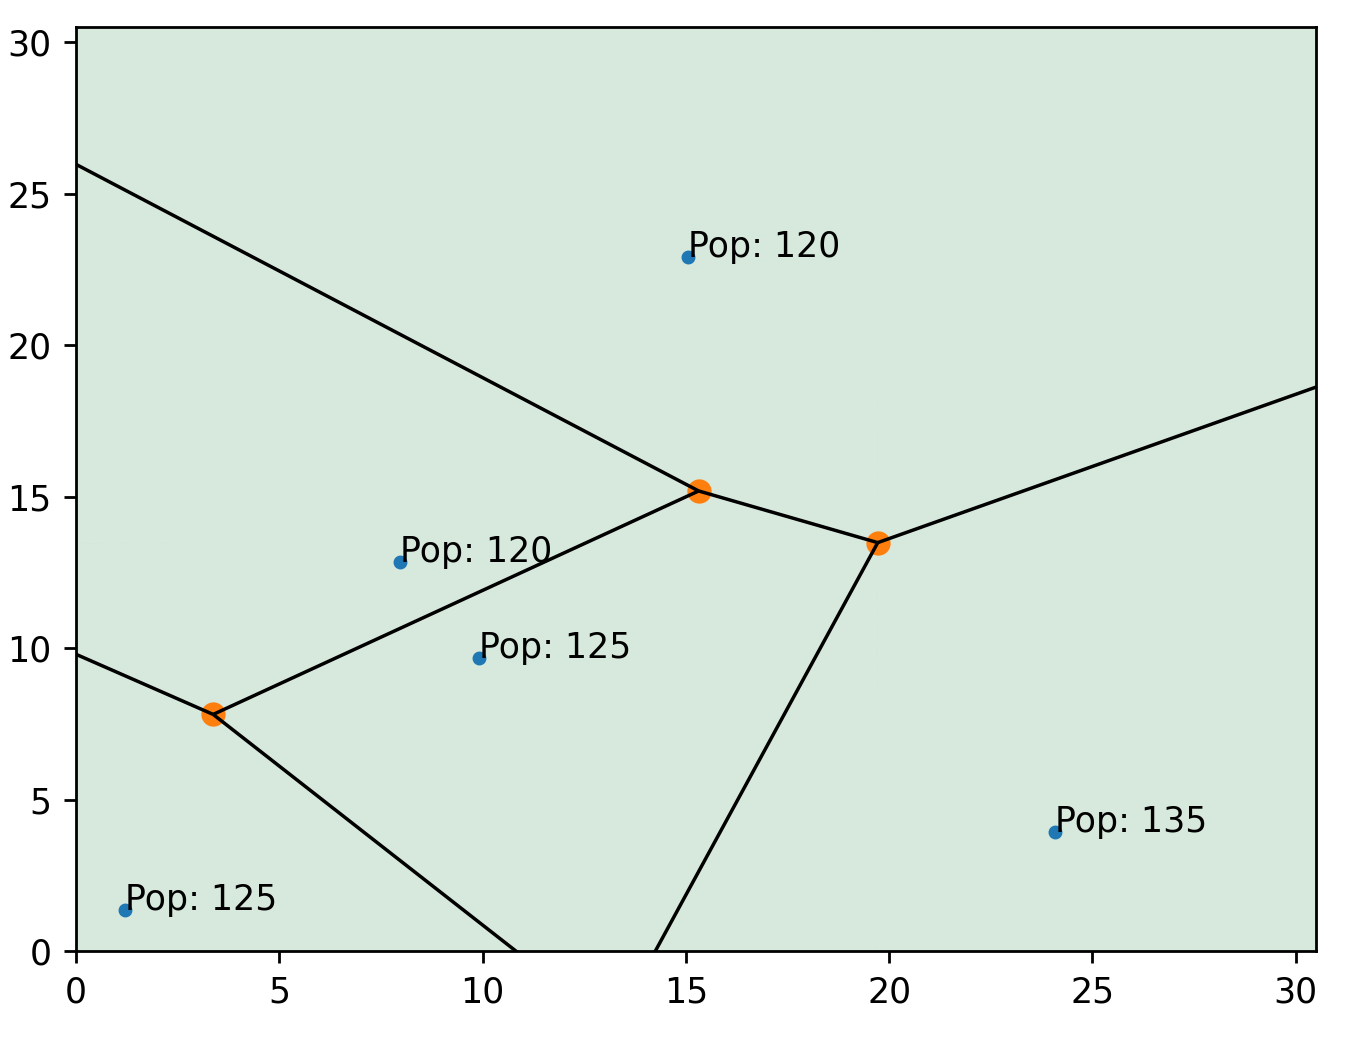
\includegraphics[clip,scale=0.16]{lim1_voronoi_60.png}
    \caption*{Approximate solution at $it = 70$}
    \label{fig:lim-1-1}
\end{figure}


However, because we are comparing facilities with each other, the facilities keep getting moved, leading the system to devolve again. 

\begin{figure}[H]
    \centering
    \captionsetup{justification=centering}
    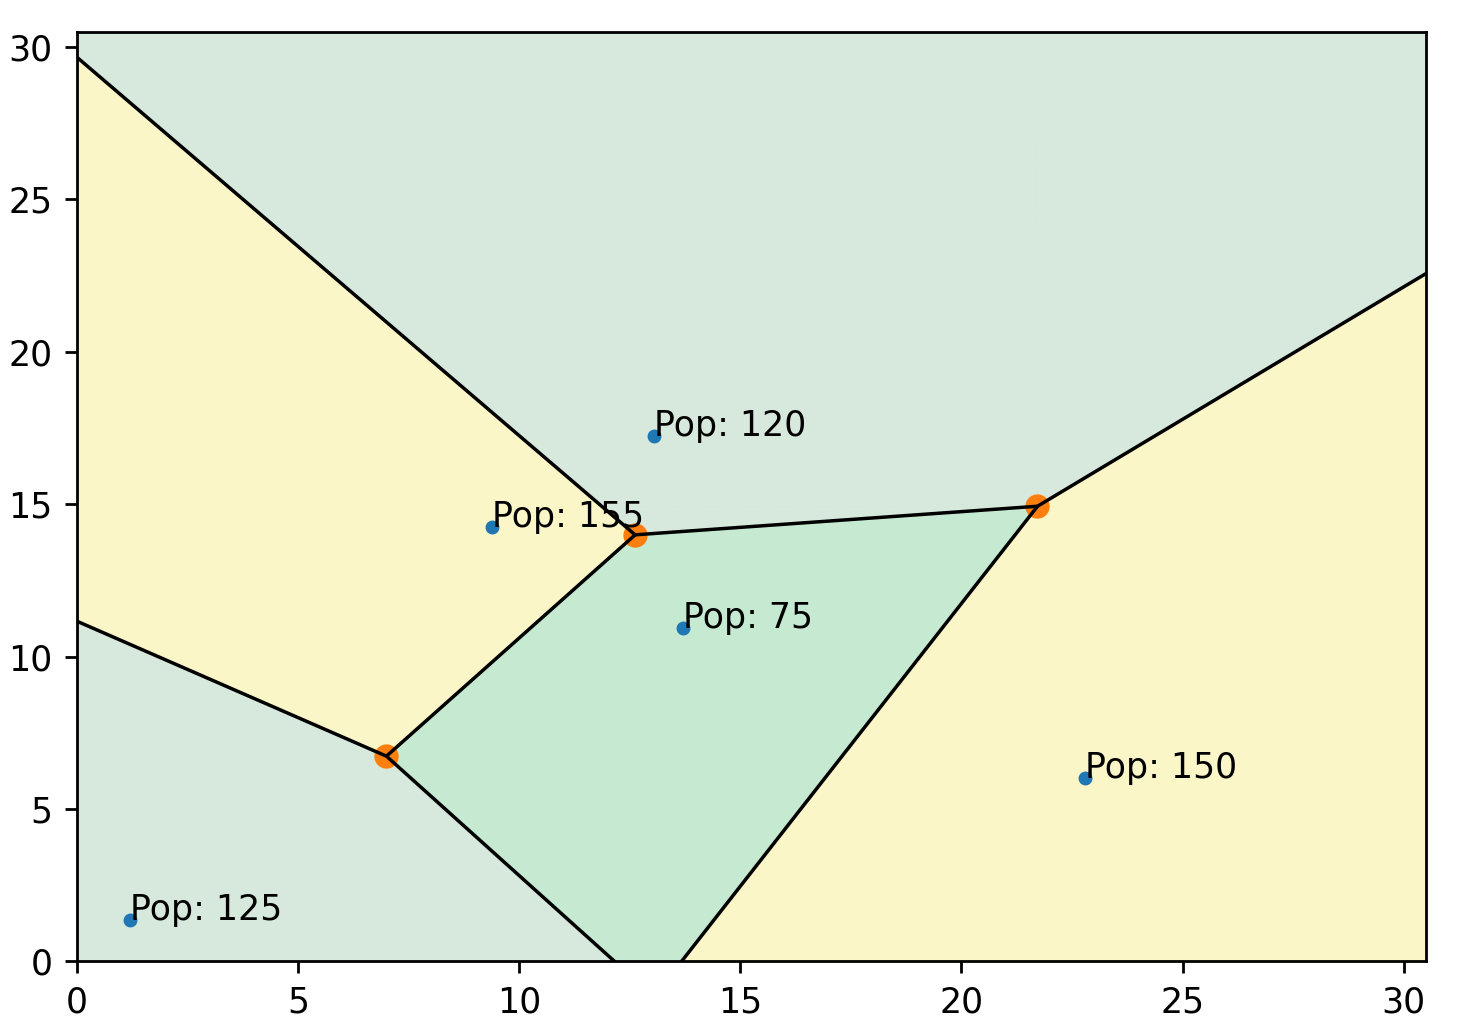
\includegraphics[clip,scale=0.16]{lim1_voronoi_110.png}
    \caption*{Approximate solution at $it = 110$}
    \label{fig:lim-1-2}
\end{figure}

\textbf{Note:} If we imagine a system where there is an overloaded facility surrounded by similarly overloaded facilities (like a pocket of overloadedness), the limiting function (1) makes it really hard to deal with that situation. 

\vspace{12pt}
If we use limiting function (2), it finds an acceptable solution at $it \approx 130$.

\begin{figure}[H]
    \centering
    \captionsetup{justification=centering, width=0.9\linewidth}
    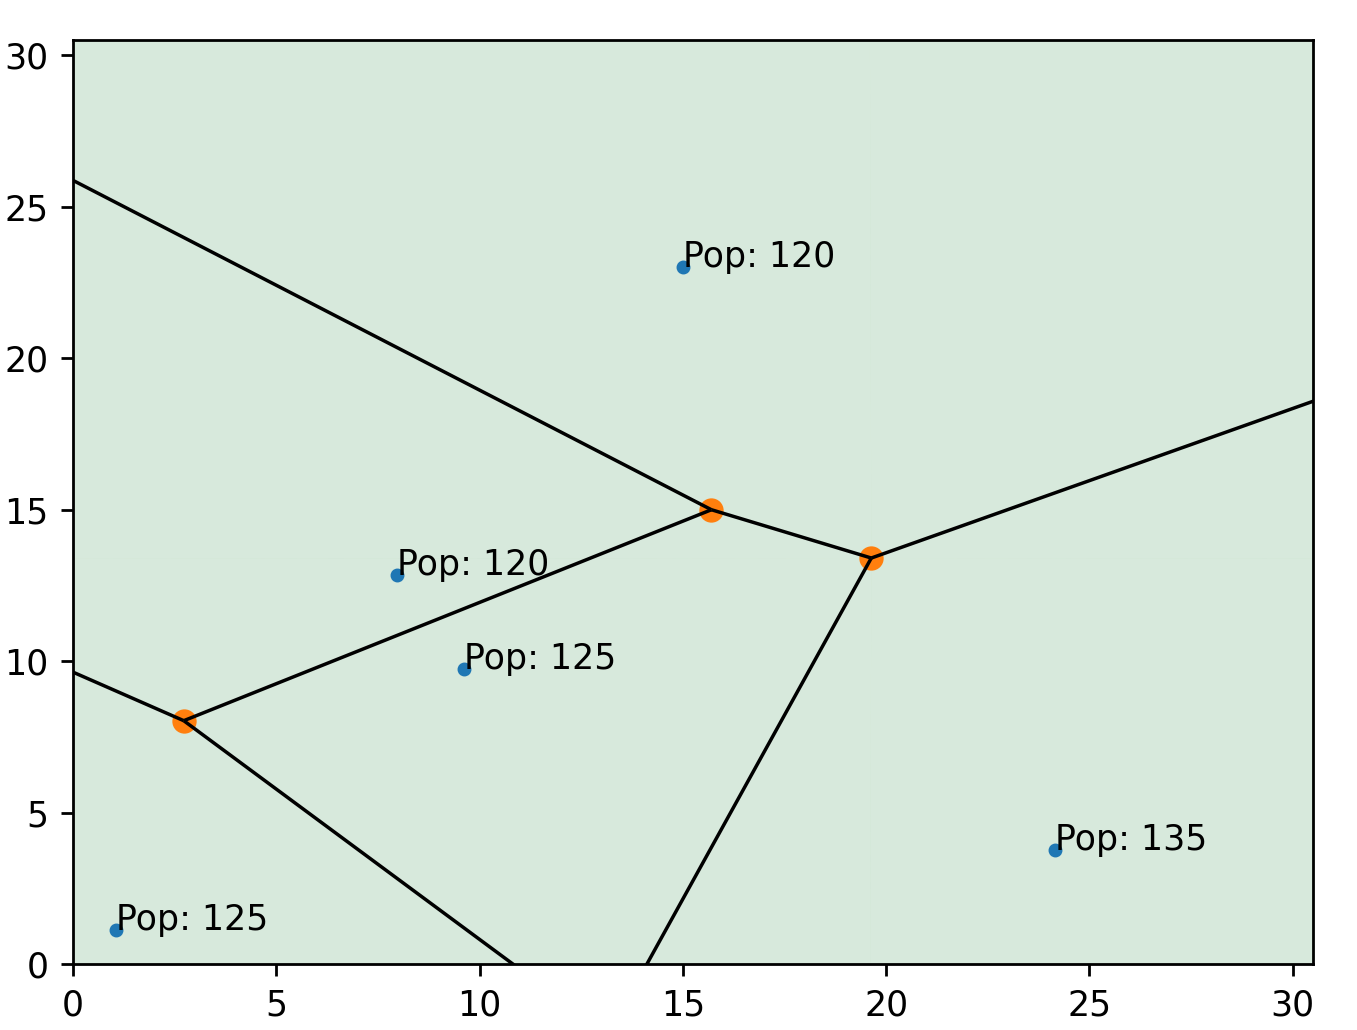
\includegraphics[clip,scale=0.16]{lim2_voronoi_140.png}
    \caption*{Approximate solution at $it = 140$ (very similar to the solution of limiting function (1) at $it = 70$)}
    \label{fig:lim-1-2}
\end{figure}

Once it hits the accepted solution because all the expected populations are within $0.9 \times avg$, all the movements resolve to $0$ and we are finished. In both methods, an issue we run into is that the techniques only ever bring facilities closer together, and sometimes we cannot find a solution. This is where algorithms need to be improved.


\begin{thebibliography}{9}
\bibitem{aha-rise}
4 Takeaways on coming shift in health services demand | AHA. (2024, July 2). American Hospital Association. https://www.aha.org/aha-center-health-innovation-market-scan/2024-07-02-4-takeaways-coming-shift-health-services-demand

\bibitem{aanp-wait}
American Association of Nurse Practitioners. (2023, July 12). Two in five Americans report unreasonable health care wait times. https://www.aanp.org/news-feed/two-in-five-americans-report-unreasonable-health-care-wait-times

\bibitem{canada-wait}
Liddy C, Moroz I, Affleck E, Boulay E, Cook S, Crowe L, Drimer N, Ireland L, Jarrett P, MacDonald S, McLellan D, Mihan A, Miraftab N, Nabelsi V, Russell C, Singer A, Keely E. How long are Canadians waiting to access specialty care? Retrospective study from a primary care perspective. Can Fam Physician. 2020 Jun;66(6):434-444. PMID: 32532727; PMCID: PMC7292524.

\bibitem{race-disparity}
Macias-Konstantopoulos, W. L., Collins, K. A., Diaz, R., Duber, H. C., Edwards, C. D., Hsu, A. P., Ranney, M. L., Riviello, R. J., Wettstein, Z. S., \& Sachs, C. J. (2023). Race, Healthcare, and Health Disparities: A Critical Review and Recommendations for Advancing Health Equity. Western Journal of Emergency Medicine, 24(5). https://doi.org/10.5811/westjem.58408

\bibitem{covid-imbalance}
Vohra, A. S., Khullar, D., Kaushal, R., & Schpero, W. L. (2023). Many intensive care units were overloaded while nearby hospitals had excess capacity during the COVID-19 pandemic. Health Affairs, 42(7), 937–945. https://doi.org/10.1377/hlthaff.2022.01657
\end{thebibliography}


\end{document}
